\documentclass[11pt,a4paper]{article}
\usepackage[margin=1in]{geometry}
\usepackage{graphicx}
\usepackage{setspace}
\usepackage{titlesec}
\usepackage{caption}

\titlespacing*{\section}{0pt}{1.2ex plus .2ex}{0.8ex plus .2ex}

\captionsetup{
  font=small,
  labelfont=bf,
  skip=4pt
}

\setstretch{1.05}

\title{\vspace{-2em}\textbf{Is Florida Getting Hotter?}\vspace{-1em}}
\author{Ekadh Ranganathan}
\date{October 2025}

\begin{document}
\maketitle
\vspace{-1em}

\section*{Results}
The mean temperature data for Florida across years shows a correlation coefficient of:
\[
r = 0.5331784
\]
This indicates that across 50{,}000 randomly shuffled samples of temperatures and years, none produced a correlation higher than the observed value. Figure 1 shows that the observed correlation lies well outside the random distribution.

\begin{figure}[h!]
\centering
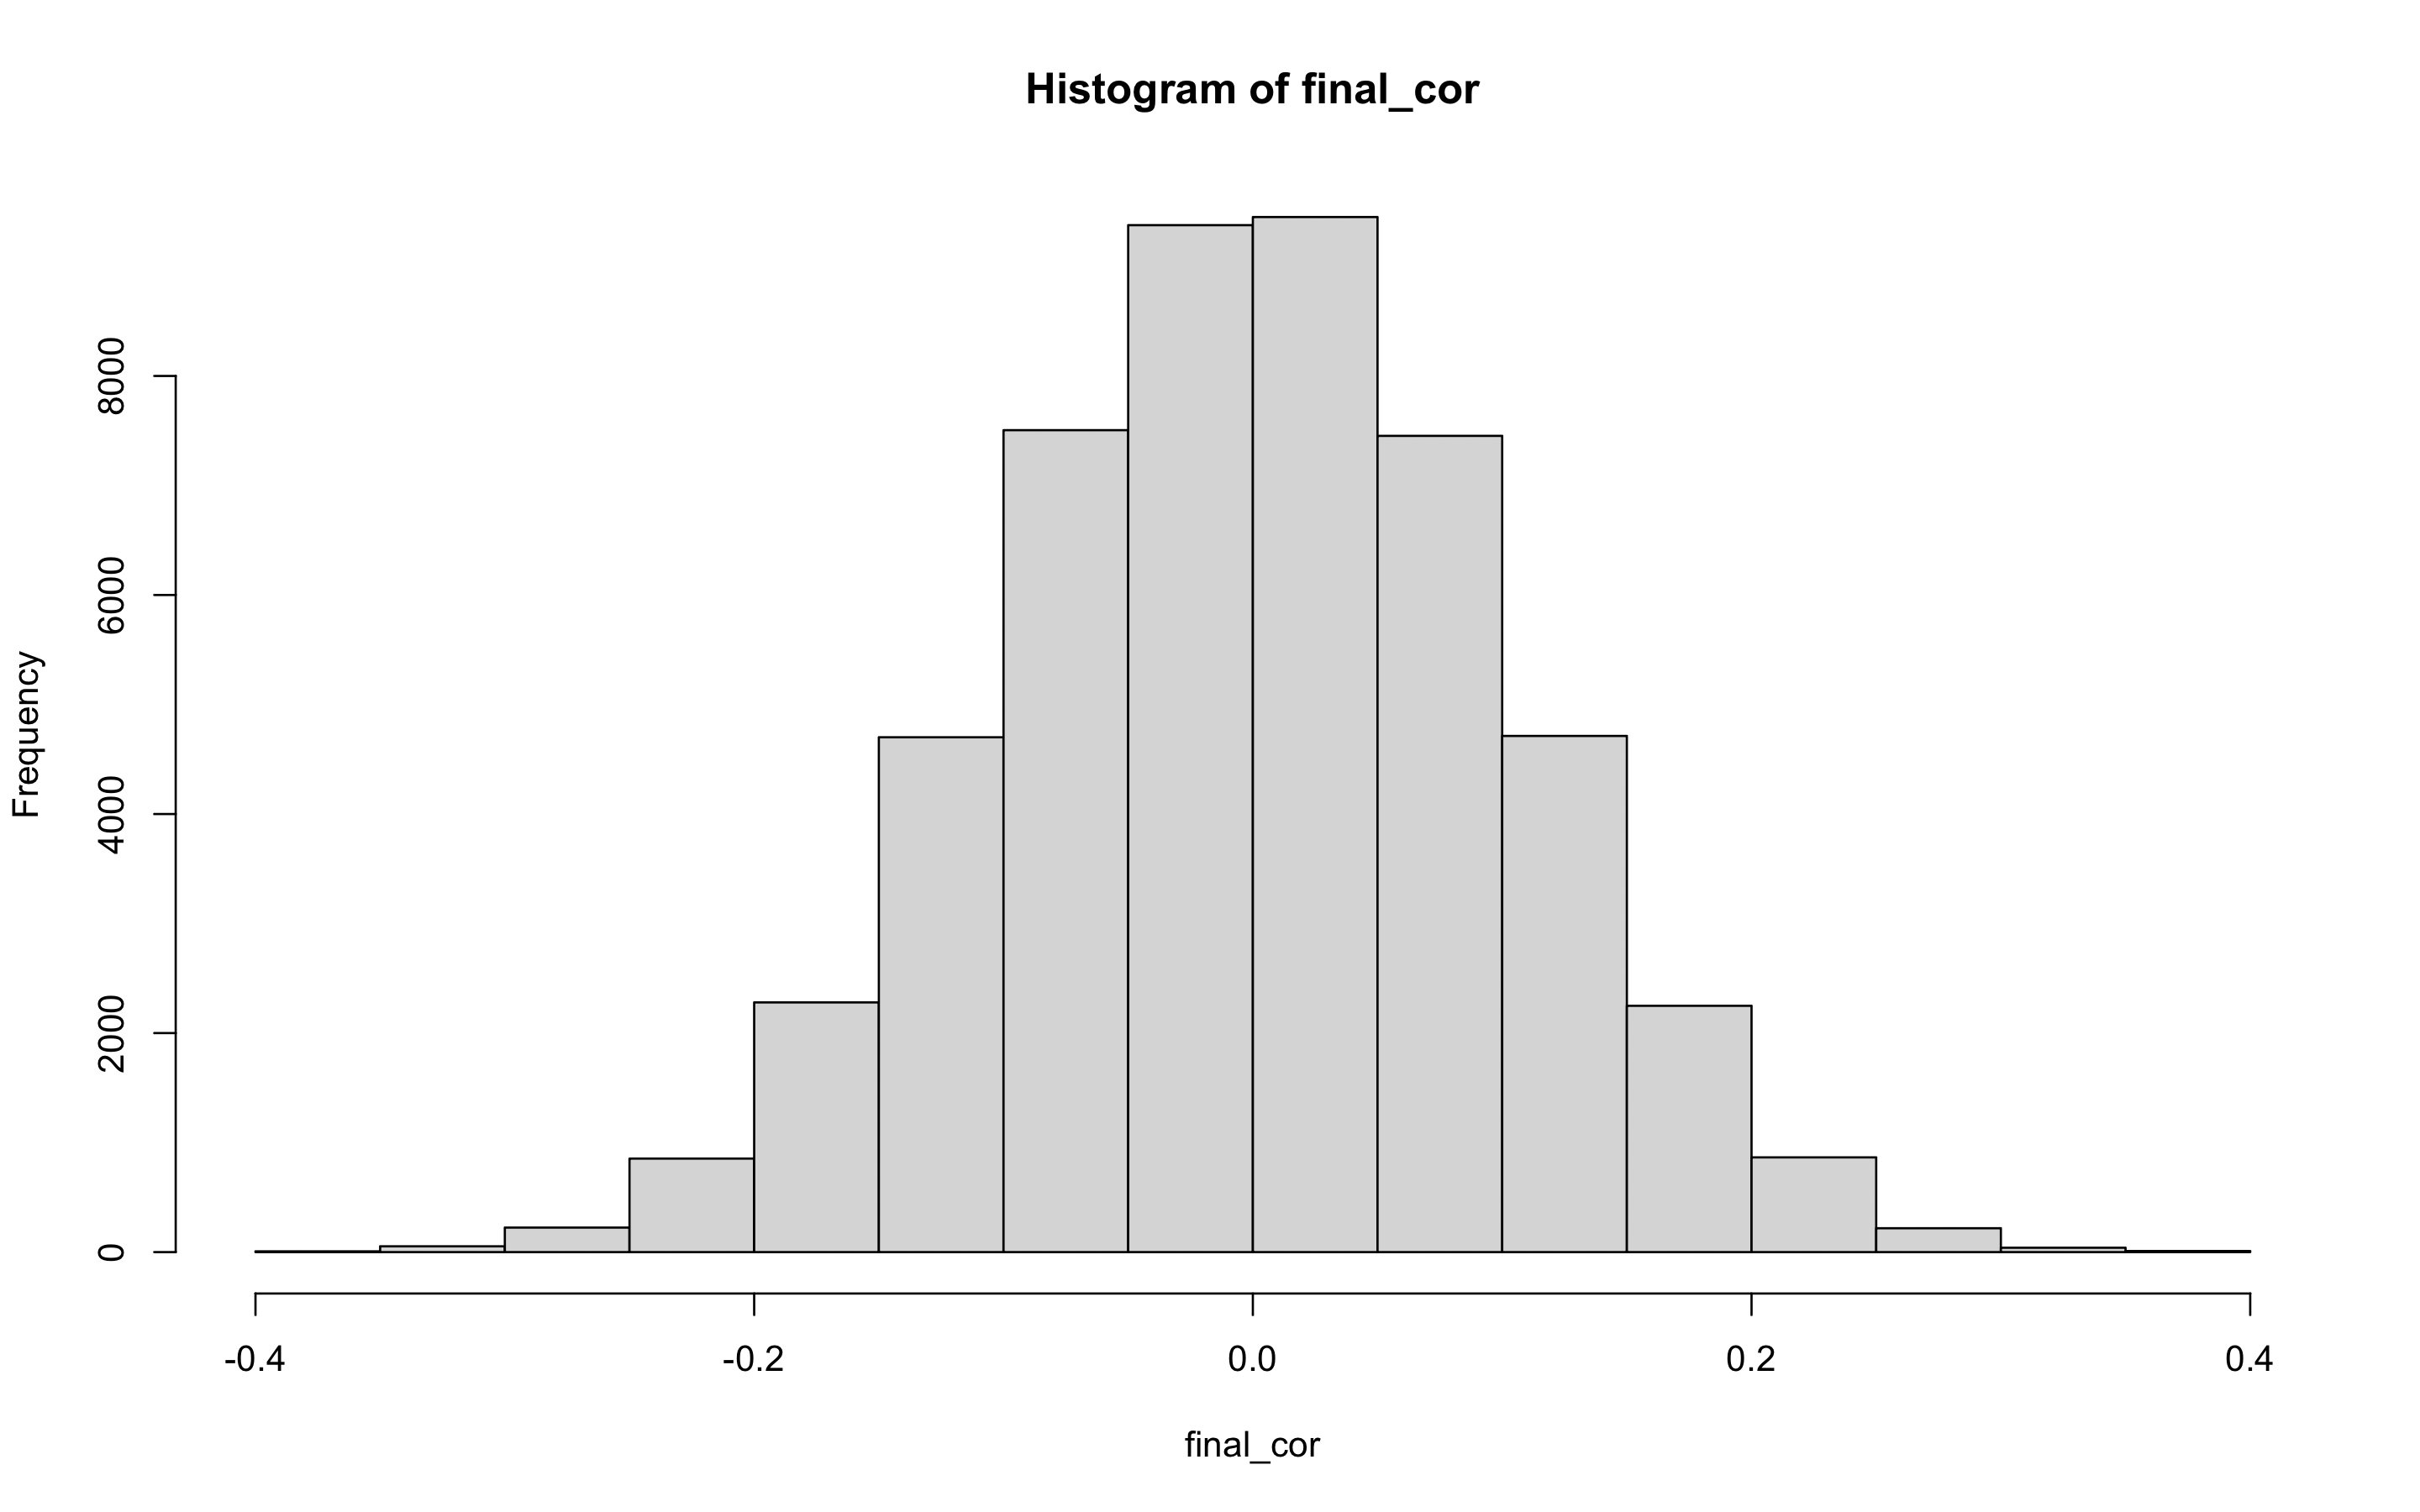
\includegraphics[width=0.6\textwidth]{../data/Histogram.png}
\caption{Distribution of correlation coefficients from 50,000 permutations. The observed Florida correlation ($r \approx 0.53$) lies outside the random range.}
\label{fig:hist}
\end{figure}

\section*{Interpretation}
The permutation analysis suggests rejecting the null hypothesis that there is no correlation between temperature and years in Key West. The p-value is less than 0.05, and since no random sample exceeded the observed correlation, the corrected p-value can be calculated as:
\[
p = \frac{1 + 0}{50{,}000 + 1} \approx 1.99996\times10^{-5}.
\]
This provides strong evidence that mean annual temperature in Florida has significantly increased over time.

\end{document}
